\section{Structural Information in Hyper-relational Knowledge Graphs}
\label{sec:background:hyperkg}

This section presents the author's published work \emph{Understanding the Embedding Models on Hyper-relational Knowledge Graph}, published at CIKM 2025~\cite{bg-hyperkg}. It examines how graph representations and embedding architectures preserve information used for link prediction. The study provides a separate perspective on structural information within the thesis. Its experiments concern KG embedding models, while the four research chapters examine language-model augmentation.

\subsection{Facts, Qualifiers, and Decomposition}

A hyper-relational fact extends a main triple with a set of qualifier pairs,
\begin{equation}
F=\left(s,r,o,\mathcal{Q}\right),\qquad
\mathcal{Q}=\{(qr_i,qe_i)\}_{i=1}^{n}.
\label{eq:background:hyper-fact}
\end{equation}
Here $qr_i$ is a qualifier relation and $qe_i$ its associated entity. Qualifiers attach information to a particular statement. For example, degree and major can distinguish two education statements about the same person. Their association with the intended main triple is part of the information represented by the fact. StarE retains the semantic roles of qualifiers and triples in message passing and introduces WD50K for hyper-relational link prediction~\cite{bg-stare}.

The CIKM study asks how much of an HKGE model's performance comes from its base KGE architecture and how much comes from specialized qualifier processing. It evaluates a data-level alternative to modifying the model. Three decomposition methods convert a hyper-relational fact into ordinary triples while retaining different information. Prune keeps only the main triple. Direct adds triples connecting the subject to qualifier entities through their qualifier relations. Hyper adds further relations whose names combine the main relation with each qualifier relation and connect the qualifier entity to the main object.

Figure~\ref{fig:background:decomposition} reproduces the original comparison, including database reification. The study distinguishes main-triple information, intra-qualifier information, and inter-qualifier information. A decomposition can retain qualifier entities and relation labels while changing how their association with the main fact is expressed. Database reification introduces auxiliary entities and relations, also changing the original main-triple topology. These differences determine which neighborhoods and paths an ordinary KGE model receives after conversion.

\begin{figure}[tbp]
\centering
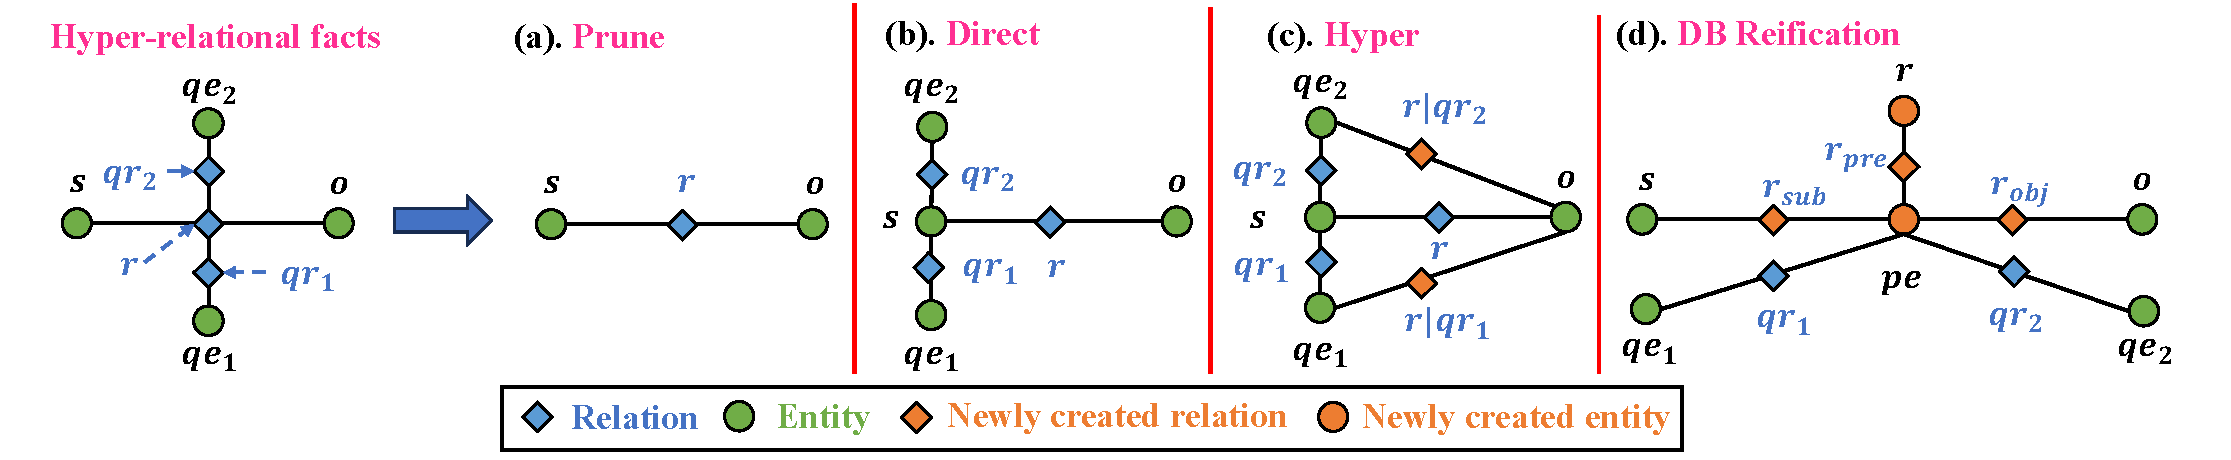
\includegraphics[width=\linewidth]{figures/hyperkg/decomp_new.pdf}
\caption{Original comparison of hyper-relational decomposition methods. Prune retains the main triple; Direct adds subject--qualifier links; Hyper adds combined relations; database reification introduces auxiliary objects. Reproduced from Fig.~1 of the CIKM study~\cite{bg-hyperkg}.}
\label{fig:background:decomposition}
\end{figure}

The association of a qualifier with a statement is especially relevant when a subject participates in several facts using the same relation. In the education example, a degree describes one university attendance statement. A collection of subject--degree and subject--university triples exposes the entities but changes the representation of which degree qualifies which attendance fact. A model following ordinary graph paths then receives the transformed connections. The Hyper method supplies additional connections intended to retain more of these associations, whereas a qualifier integrator receives the main fact and its qualifier pairs together. This comparison places information preservation at the interface between the data representation and the computation that follows it. It concerns the semantic organization of the input as well as its vocabulary.

The experiments compare conventional KGE models under these transformations with specialized HKGE models. Some GNN-based KGE configurations obtain scores comparable to specialized methods on Cleaned JF17k and WD50k. The observation motivates an examination of the represented information and the architecture receiving it. In particular, adding qualifier-derived edges can change the paths followed by a graph encoder. Preserving more items in a converted graph therefore changes the model's computational input as well as the nominal amount of stored information.

\subsection{Qualifier Capture and Graph Reception}

The analysis separates qualifier capture from graph reception. Qualifier capture concerns how the model represents qualifier pairs and their association with the main statement. Graph reception concerns how it receives information from the wider graph, including dependencies beyond one fact. Models operating on a fact in isolation have a different receptive field from graph encoders that propagate information across several hops. These properties are visible in the operations used to construct representations.

CompGCN jointly models entity and relation representations in a multi-relational graph~\cite{bg-compgcn}. NBFNet aggregates path information for link prediction~\cite{bg-nbfnet}. Their graph computations offer different ways to receive neighborhood and path information after decomposition. The CIKM analysis also identifies an information-compression issue when qualifier information is aggregated into fixed-size main-triple representations. Wider graph reception and qualifier integration consequently concern complementary parts of the architecture. The study evaluates designs that retain both sources for prediction.

FormerGNN combines a Transformer-based qualifier integrator operating on the original hyper-relational facts with a graph encoder operating on the pruned main-triple graph. The graph encoder generates a topology representation for the subject. The model concatenates this representation with representations of the main triple and qualifier pairs and passes them to a Transformer decoder. This organization supplies qualifier and graph information jointly to the prediction stage. In the reported configuration, HyperFormer provides the qualifier integrator and NBFNet provides the graph encoder~\cite{bg-hyperformer,bg-nbfnet}.

\subsection{Representative Published Evidence}

Table~\ref{tab:background:formergnn} reproduces the Cleaned JF17k and WD50k columns of the study's Table~6. It retains all seven model rows and all three metrics for those datasets. MRR measures mean reciprocal rank, and H@1 and H@10 measure whether the target entity appears within the corresponding rank cutoff. These are link-prediction measures, distinct from the annotation and answer metrics of the later chapters.

\begin{table}[tbp]
\centering
\caption{Projection of the CIKM study's Table~6 onto Cleaned JF17k and WD50k. All model rows and the original metric precision are retained; the original bold and underline markings indicate best and second-best values.}
\label{tab:background:formergnn}
\small
\begin{tabular}{lrrrrrr}
\toprule
&\multicolumn{3}{c}{Cleaned JF17k}&\multicolumn{3}{c}{WD50k}\\
\cmidrule(lr){2-4}\cmidrule(lr){5-7}
Model&MRR&H@1&H@10&MRR&H@1&H@10\\
\midrule
StarE&0.381&0.284&0.577&0.346&0.268&0.494\\
QUAD&0.402&0.305&0.602&0.349&0.275&0.487\\
HAHE&0.405&0.310&0.585&0.360&0.288&0.496\\
HyperFormer&\underline{0.425}&\underline{0.328}&0.613&\underline{0.372}&\underline{0.293}&0.522\\
NBFNet + Prune&0.415&0.313&\textbf{0.630}&0.360&0.271&\textbf{0.530}\\
CompGCN + Hyper&0.389&0.294&0.590&0.350&0.277&0.488\\
FormerGNN&\textbf{0.432}&\textbf{0.335}&\underline{0.624}&\textbf{0.377}&\textbf{0.299}&\underline{0.527}\\
\bottomrule
\end{tabular}
\end{table}

FormerGNN obtains MRR 0.432 on Cleaned JF17k and 0.377 on WD50k, compared with HyperFormer's 0.425 and 0.372. NBFNet + Prune has the highest H@10 in both selected datasets, at 0.630 and 0.530. The table therefore supports a metric-specific comparison. The experiment uses a single NVIDIA A100-40GB GPU. Parameters follow the original repositories or are selected by grid search when dataset-specific settings are unavailable. For comparisons involving CompGCN, the study replaces its decoder with a Transformer to align it with the corresponding HKGE configurations.

The complete published comparison also includes Wikipeople and FBAUTO, where dataset characteristics and metric rankings differ. The selected table illustrates the result associated with the main discussion of graph reception and qualifier integration; it is not an average over the four datasets. The research establishes that the organization of graph information can matter beyond retaining the same entity and relation vocabulary. Its connection to this thesis is the design question of which relationships remain available to a model after evidence transformation. FormerGNN is a separate KG embedding framework; the four language-model systems use the structures and interfaces defined in their own chapters.

